\documentclass[a4paper]{article}

\usepackage[top=3cm, bottom=2cm, left=2cm, right=2cm]{geometry}
\usepackage{graphicx}
\usepackage{fancyhdr}
\usepackage{scrextend}
\usepackage[hidelinks]{hyperref}
\usepackage{textcomp}
\usepackage{tipa}
\usepackage{caption}
\usepackage{subcaption}

\graphicspath{ {./images/} }

\title{Homework 2 - Machine Learning: Weather Classification}
\author{Edoardo Piroli - 1711234}

\pagestyle{myheadings}
\pagestyle{fancy}
\fancyhf{}

\renewcommand{\headrulewidth}{0pt}
\renewcommand{\footrulewidth}{1pt}

\fancyfoot[C]{Report HW2 - Machine Learning}
\fancyfoot[R]{\thepage}

\begin{document}

\maketitle
\thispagestyle{empty}

\newpage
\tableofcontents
\thispagestyle{empty}
\newpage

\pagenumbering{arabic}

\section{Introduction}
\subsection{Assignment}
The assignment of the homework was to build an image classifier capable of assigning pictures to one of the following classes: \{\textit{RAINY}, \textit{HAZE}, \textit{SUNNY}, \textit{SNOWY}\}; based on how the weather was like at moment of the picture's capture. In particular, the request was to address the former problem in 2 different ways: 
\begin{enumerate}
\item Defining and training a CNN from scratch for this particular task;
\item Applying transfer learning and fine-tuning on a pre-trained model.
\end{enumerate}
\subsection{Dataset}
The provided datasets\footnote{available here: \href{https://drive.google.com/drive/folders/1UzH28Q8xki8_DMYdDgHxi40-CJ800Kaq}{https://drive.google.com/drive/folders/1UzH28Q8xki8\textunderscore DMYdDgHxi40-CJ800Kaq}} are separated in several different archives and folders. I have chosen to use \textit{MWI-Dataset-1.1\textunderscore 2000}. It contains 500 different pictures for each class and I have divided it into training and testing datasets, with the former containing 85\% of the pictures and the latter the remaining ones.

\paragraph{Chosen resolution}
In order to train both the new CNN and the pre-trained model I have resized all the pictures to a fixed resolution of 160x160. However simply resizing the pictures would've ended up radically changing the aspect ratio of the non-square ones, potentially leading to the distortion of the information contained in them. That's why, for each picture, I have resized the longest side to 160, keeping constant the aspect ratio; i.e. proportionately resizing also the other side; and pasted the so-obtained picture on a black 160x160 square: basically adding some padding to the edges. 

As an example of this resizing process here is one sample picture:

\begin{figure} [h!]
\centering
\begin{subfigure}{0.5\textwidth}
  \centering
  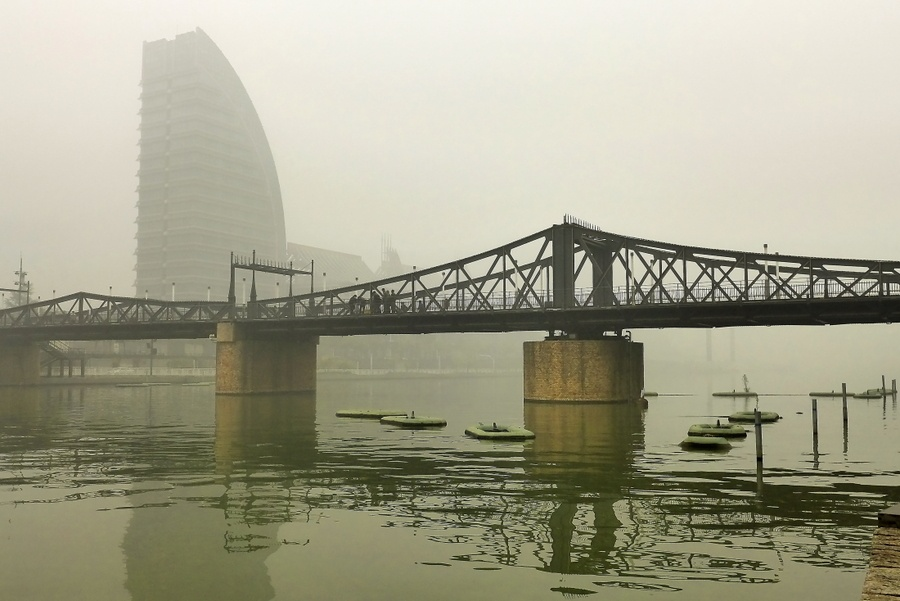
\includegraphics[width=0.99\textwidth]{HAZE-1-1-1_001_ORI.jpg}
  \caption{Original picture with resolution 900x601}
  \label{fig:sub1}
\end{subfigure}%
\begin{subfigure}{0.5\textwidth}
  \centering
  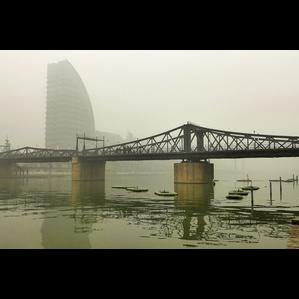
\includegraphics[width=0.99\textwidth]{HAZE-1-1-1_001_ORI_resized.jpg}
  \caption{Resized picture with resolution 160x160}
  \label{fig:sub2}
\end{subfigure}
\label{fig:test}
\end{figure}

\paragraph{Notes} Due to the limited computing power I have just chosen 160x160 as the resolution of pictures instead of actually studying the effect of this hyperparameter via, for example, Random Search. 

Similarly, instead of running cross validation, I have randomly sampled the training and testing datasets once.
\newpage
\section{Experimentation}
\subsection{Framework}
\end{document}